
%%%
% Discuss how neighboring weights were applied and what the results were
% TODO: results
%%%

\subsubsection{Neighboring Weights}
\label{sec:findings-expts-neighbors}

%%%
% Process
%%%

%%%
In order to smooth out the strategy graphs
and prevent isolated states of separate weights,
a blending of neighboring weights was developed.
%
Rather than simply take the set of weights allocated to a single score location,
the agent instead takes a weighted average of all surrounding weight vectors
with its own location.
%
In other words,
\[
    w'_{m,o,d} = %\mathrm{l1norm}\left(
    \left|
    Xw_{m,o,d} +
    Y \sum_{i\in\{-1,0,1\}} \sum_{j\in\{-1,0,1\}} w_{m+i,o+j,d}
    \right|_1
    %\right)
\]
where $X$, $Y$ are ratios of each vector's effect, $X+Y = 1$,
and $m+i$, $o+j \in [0,120]$.
%
The desired effect was to allow a score location to learn from its neighbors
so that a neighborhood effect was present in the decision.
%%%


\paragraph{Results}

%%%
% Results:
%	Mostly same appearnace
%	fewer islands in hand_max_min territory for cribminavg/peggingminavggiven/
%		peggingmaxmedgained/peggingmaxavggained
%	Losing territory still in limbo, not much certainty there.
%%%

%%%
% Not really good at making a blending/gradient
% Definitely did eliminate islands though
%%%


\begin{figure}
\center

	\begin{subfigure}[t]{0.22\textwidth}
		\center
		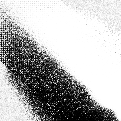
\includegraphics[width=\stratgraphwidth]{images/findings/experiments/neighbors/strats/hand_max_min.png}
		\caption{\handmaxmin}
	\end{subfigure}
	~
	\begin{subfigure}[t]{0.22\textwidth}
		\center
		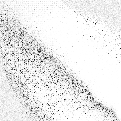
\includegraphics[width=\stratgraphwidth]{images/findings/experiments/neighbors/strats/hand_max_avg.png}
		\caption{\handmaxavg}
	\end{subfigure}
~
	\begin{subfigure}[t]{0.22\textwidth}
		\center
		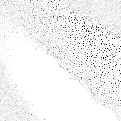
\includegraphics[width=\stratgraphwidth]{images/findings/experiments/neighbors/strats/hand_max_med.png}
		\caption{\handmaxmed}
	\end{subfigure}
	~
	\begin{subfigure}[t]{0.22\textwidth}
		\center
		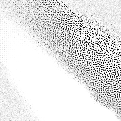
\includegraphics[width=\stratgraphwidth]{images/findings/experiments/neighbors/strats/hand_max_poss.png}
		\caption{\handmaxposs}
	\end{subfigure}

	\begin{subfigure}[t]{0.22\textwidth}
		\center
		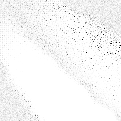
\includegraphics[width=\stratgraphwidth]{images/findings/experiments/neighbors/strats/crib_min_avg.png}
		\caption{\cribminavg}
	\end{subfigure}
	~
	\begin{subfigure}[t]{0.22\textwidth}
		\center
		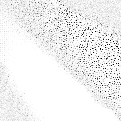
\includegraphics[width=\stratgraphwidth]{images/findings/experiments/neighbors/strats/pegging_max_avg_gained.png}
		\caption{\peggingmaxavggained}
	\end{subfigure}
~
	\begin{subfigure}[t]{0.22\textwidth}
		\center
		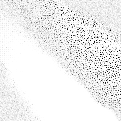
\includegraphics[width=\stratgraphwidth]{images/findings/experiments/neighbors/strats/pegging_max_med_gained.png}
		\caption{\peggingmaxmedgained}
	\end{subfigure}
	~
	\begin{subfigure}[t]{0.22\textwidth}
		\center
		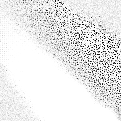
\includegraphics[width=\stratgraphwidth]{images/findings/experiments/neighbors/strats/pegging_min_avg_given.png}
		\caption{\peggingminavggiven}
	\end{subfigure}

\caption{
	Final strategy graphs for an agent when playing as the dealer
	after being trained for 500,000 games
	by following a policy which uses a weighted sum of neighboring weights.
}
\label{fig:neighbor-strats}
\end{figure}


%%%
Perhaps unfortunately,
the agent was not capable of weighting the different strategies in a
gradient-like manner
by using the neighboring score locations' weights vectors.
%
In fact,
the \handmaxavg\ strategy,
which one would expect most to form a gradient with and around the
\handmaxmin\ strategy,
was perhaps the most negatively affected.
%
As seen in Figure~\ref{fig:ex-neigh-blah},
the \handmaxavg\ strategy graph has become more sparse in the winning
triangle
with very little gray area surrounding the black.
%%%

%%%
Interestingly,
while the neighboring weights did not solidify any presence in the graphs,
the new training method did make progress in negative space.
%
This is to say that
the weighted neighbors learning method eliminated the usually present islands
of a single strategy within a swathe of another dominant strategy.
%
This white-space was present in both the winning and losing triangles.
%
This finding leads to the conclusion that weighted learning techniques
do indeed allow for a sharing of knowledge between like states,
but only insofar as to know what not to do.
%%%

%%%
Furthermore,
there is still a vast degree of uncertainty present in the losing triangles of
the strategy graphs.
%
The hope that the certainty of the winning triangle might potentially
\textit{bleed} over into the losing side was not demonstrated over the course of
the first half million training games.
%
However,
since the elimination of islands shows an improvement in
preventing lucky happenstance dictate a space's future,
the neighboring weights training method has shown usefulness in training a
cribbage agent in which states neighboring states are often similar in nature.
%%%

